\section{ 与中断相关的知识点 }
\subsection{ 中断开启和关闭函数 }
\begin{itemize}
    \item 中断开启函数:void attachInterrupt(参数一,参数二,参数三).参数一表示要为哪一个引脚开启中断;参数二表示中断触发时要调用哪个函数(填入函数指针);参数三为触发中断的方式
        \begin{table}[h]
    \centering
    \begin{tabular}{|l|l|}
    \hline
    \textbf{宏定义} & \textbf{含义} \\
    \hline
    \texttt{RISING}  & 上升沿触发（低$\rightarrow$高） \\
    \hline
    \texttt{FALLING} & 下降沿触发（高$\rightarrow$低） \\
    \hline
    \texttt{CHANGE}  & 电平变化时触发 \\
    \hline
    \texttt{LOW}     & 低电平触发 \\
    \hline
    \texttt{HIGH}    & 高电平触发（ESP32支持，Arduino Uno不支持） \\
    \hline
    \end{tabular}
    \caption{attachInterrupt 触发方式}
    \end{table}
    \item 中断关闭函数:void detachInterrupt(参数一),参数一表示要将哪个引脚的中断功能关闭
\end{itemize}
具体说明如下:
\begin{figure}[h]
    \begin{minipage}{0.48\textwidth}
        \centering
        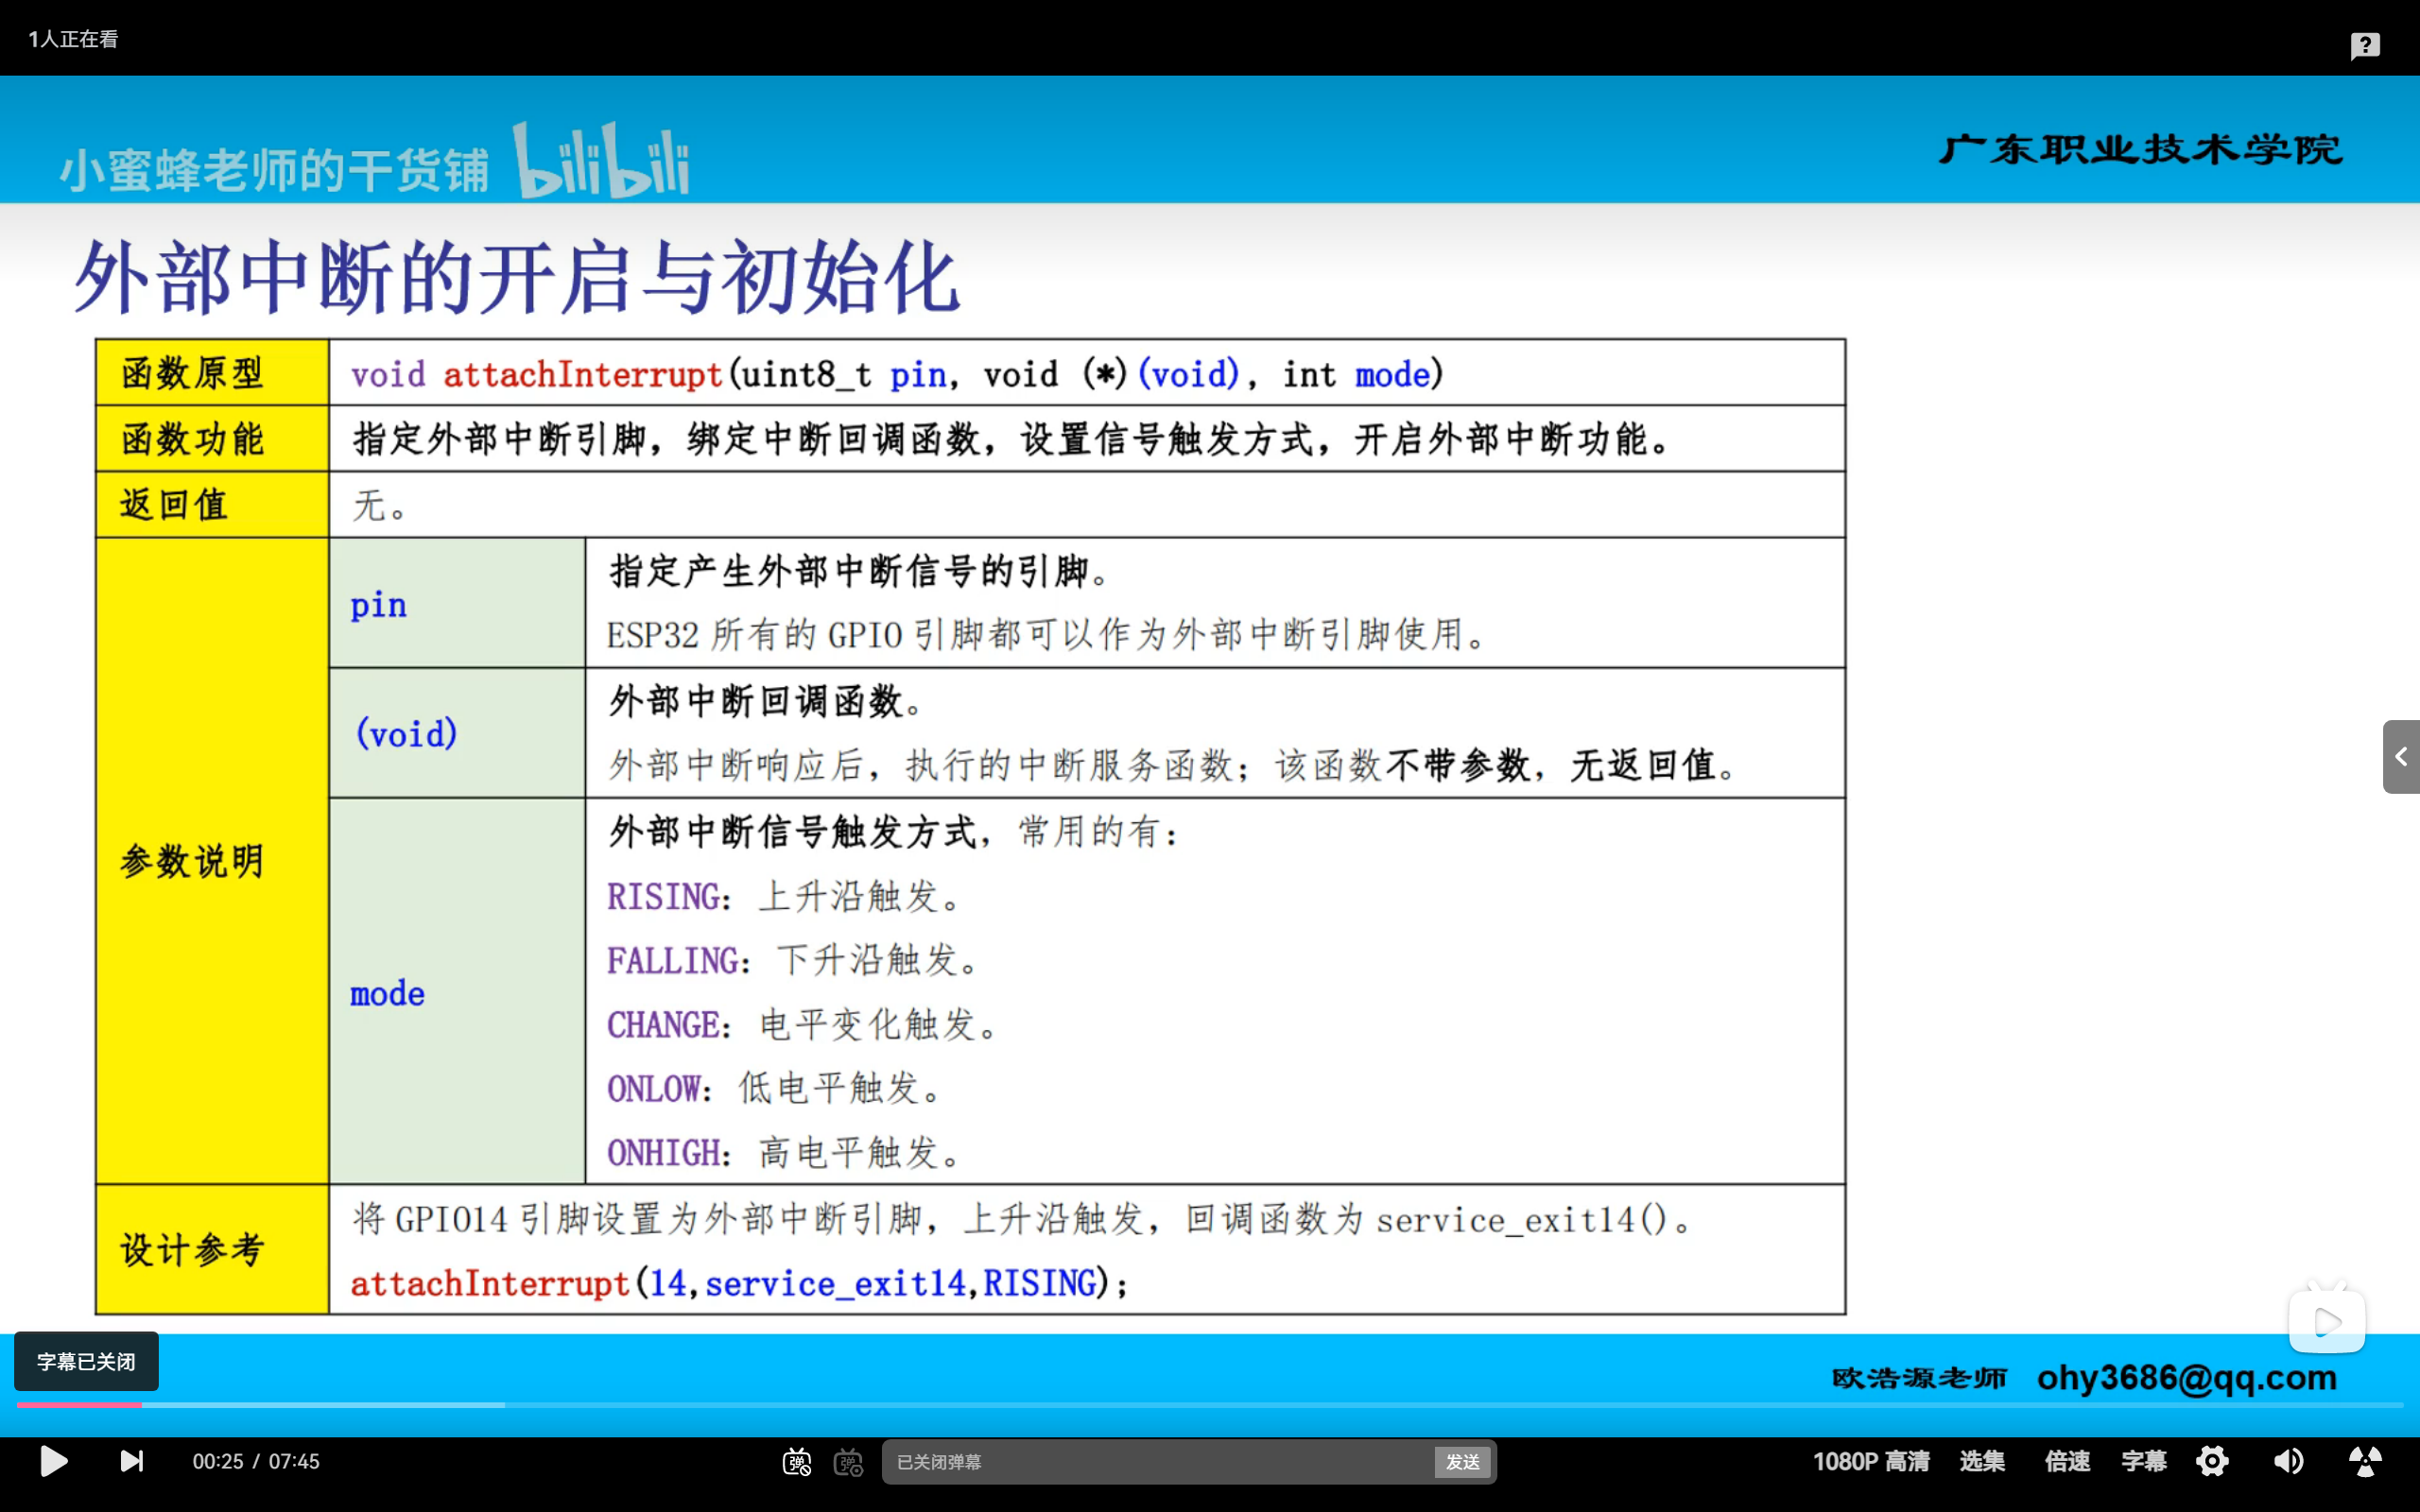
\includegraphics[width = 0.8\textwidth]{Figures/PreInterrupt.png}
        \caption{外部中断开启函数}
    \end{minipage}
    \begin{minipage}{0.48\textwidth}
        \centering
        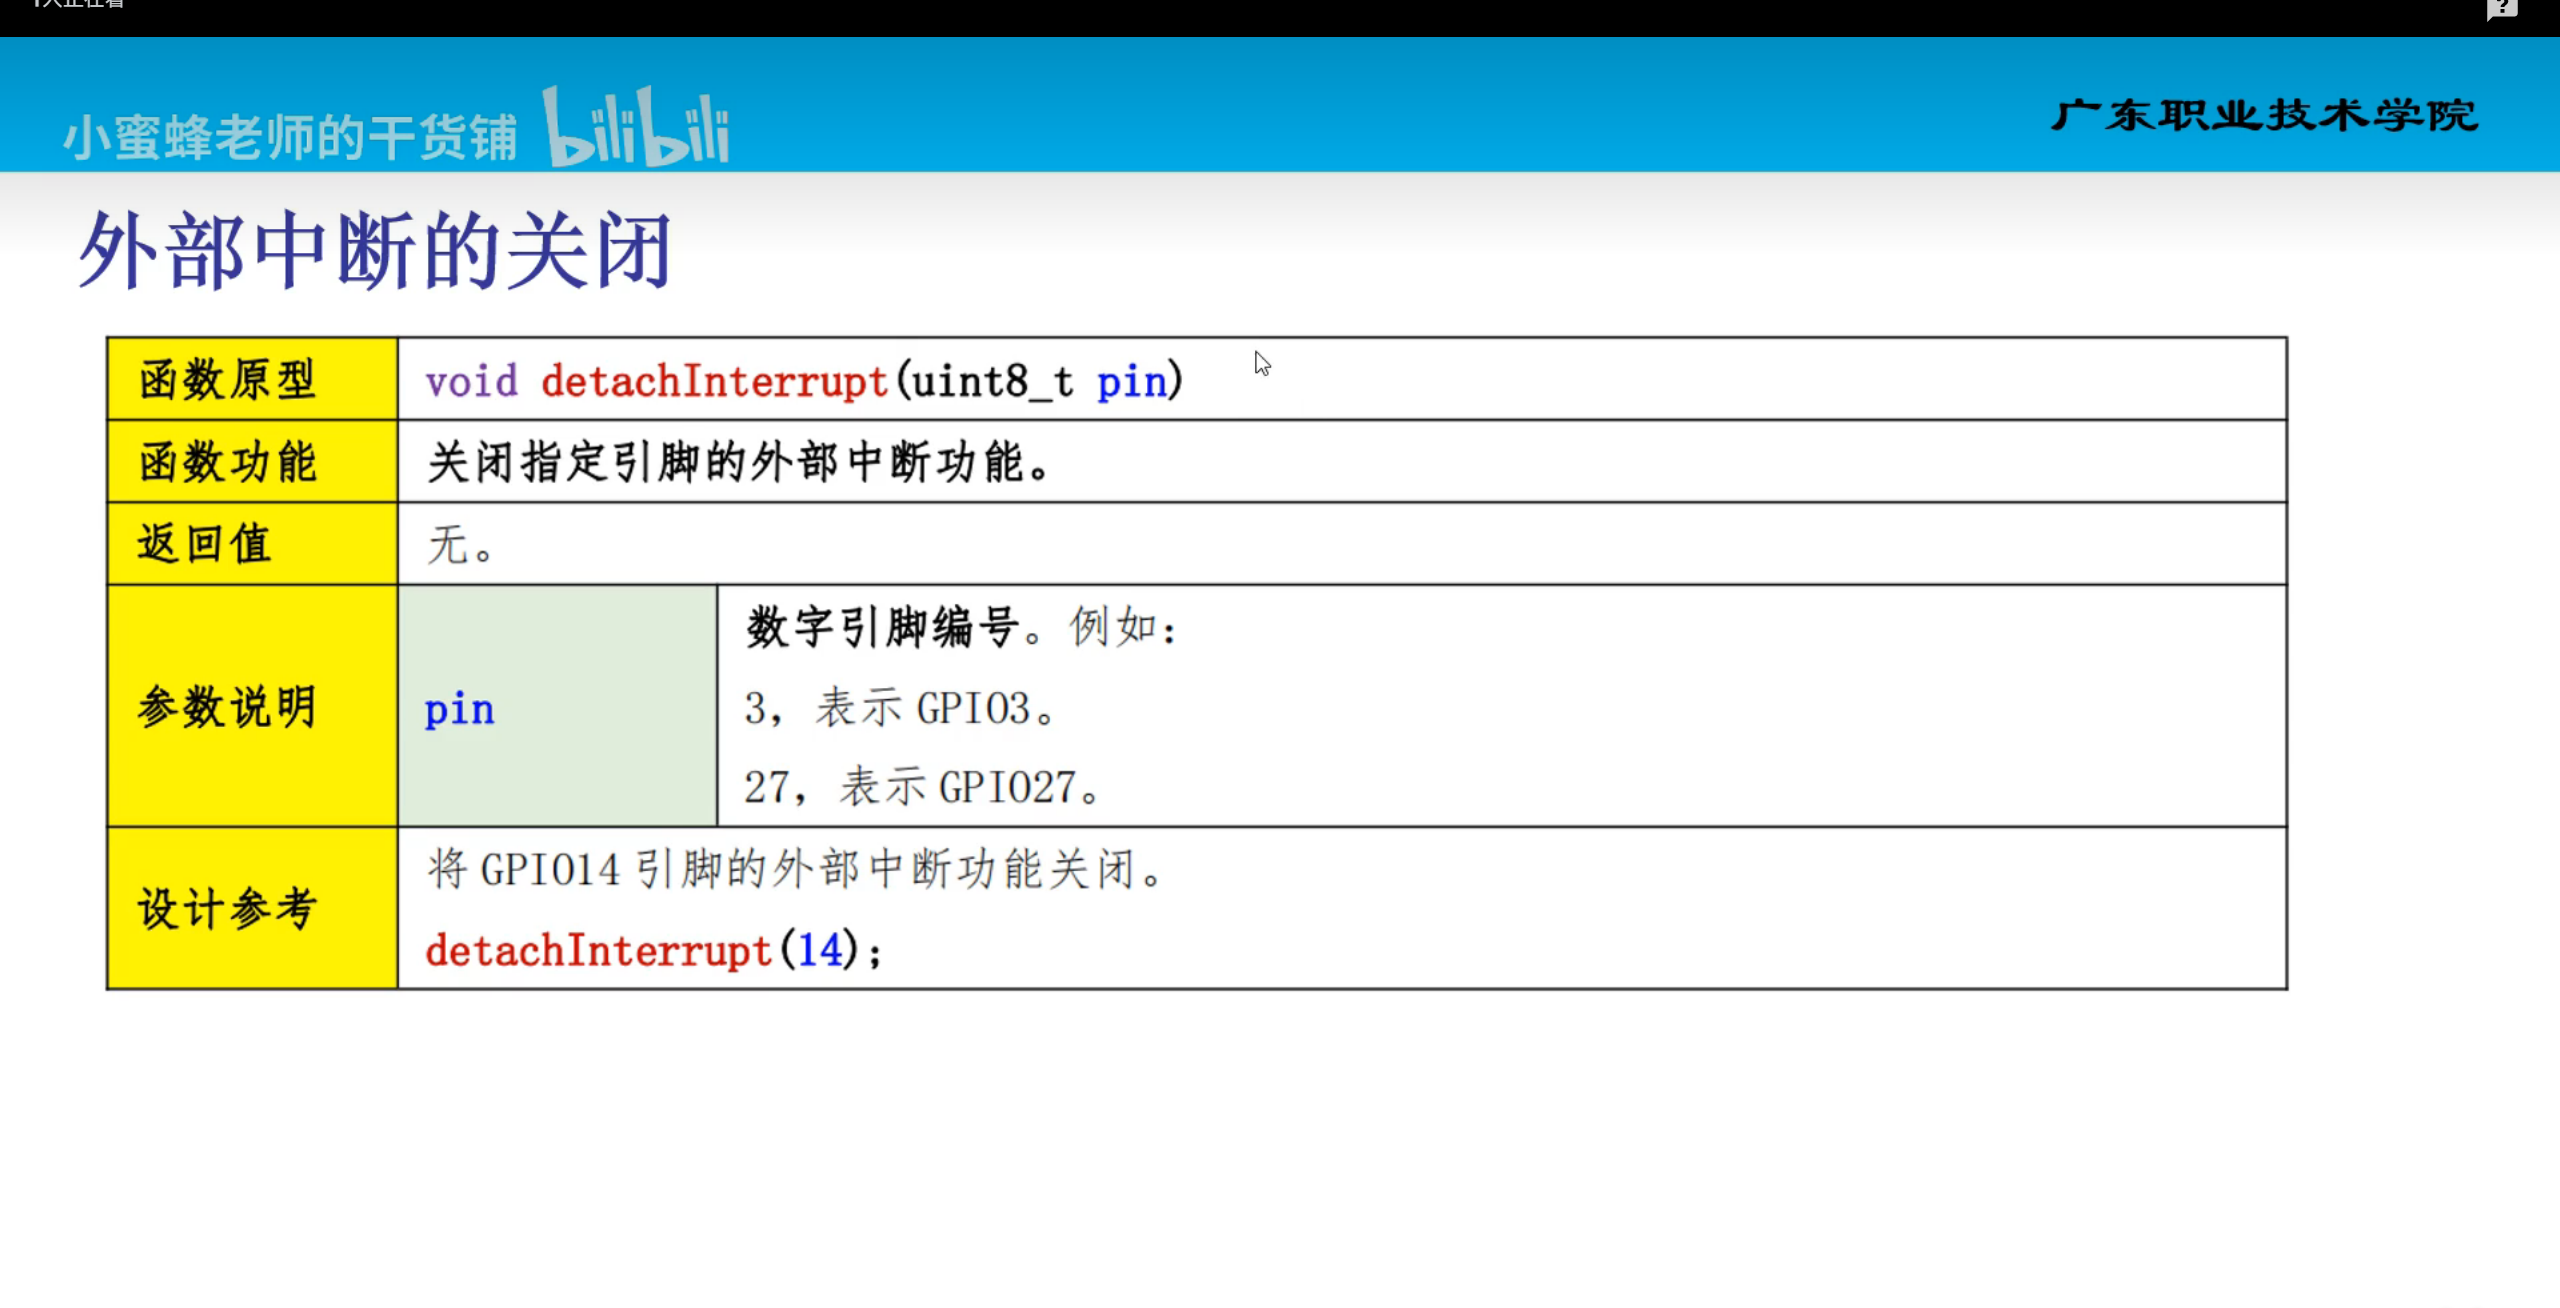
\includegraphics[width = 0.8\textwidth]{Figures/PreInterrupt_Close.png}
        \caption{外部中断关闭函数}
    \end{minipage}
\end{figure}
以下是具体的代码示例:
\begin{figure}[h]
    \centering
    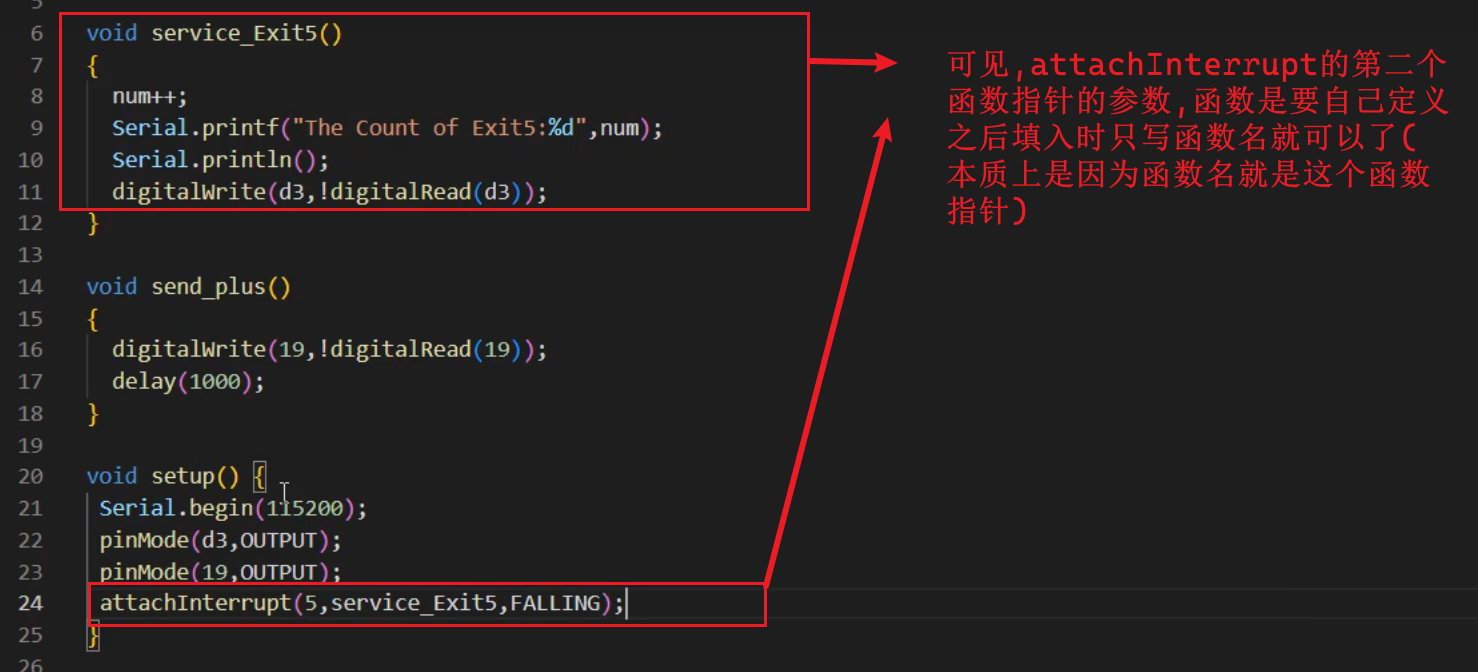
\includegraphics[width=0.5\textwidth]{Figures/Exemple_Code.png}
    \caption{外部中断开启的示例代码}
\end{figure}
